\section{Notation and problems}
\label{sec:prelim}

\noindent
\textbf{Network and disease model} (summarized in Table \ref{tab:notation}).
Let $G = (V, E)$ be a contact graph where $V$ is the set of people (or nodes) and $e = (u, v) \in E$ if nodes $u, v \in V$ come into direct contact, which can allow a disease to spread. Let $n = |V|$ be the number of nodes in graph $G$. 
We assume a simple SIR model of disease spread \cite{marathe:cacm13}, in which each node is in one of the following states:
susceptible (S), infectious (I) or recovered (R).
The epidemic starts at one or more externally infected nodes, and spreads from an infected node $u$ to each susceptible
neighbor $v$ with probability $p$. An infected node becomes recovered in the next time step.
We assume $s_v$ is the probability that $v$ is initially infected; $\mathbf{s}$ denotes the initial infection vector.
As is typical in public health analyses, we will assume a small number of random initial infections.\\
\textbf{Note.} The SIR model generalizes the well studied \emph{independent cascades} model \cite{kempe:kdd03}.
Also, there are lots of variations of the SIR model, such as:
varying transmission probability $p(u, v)$ on each edge $(u, v)$,
with an exposed state, varying infectious duration, etc.;
most of our results extend to the general models.

\begin{figure}
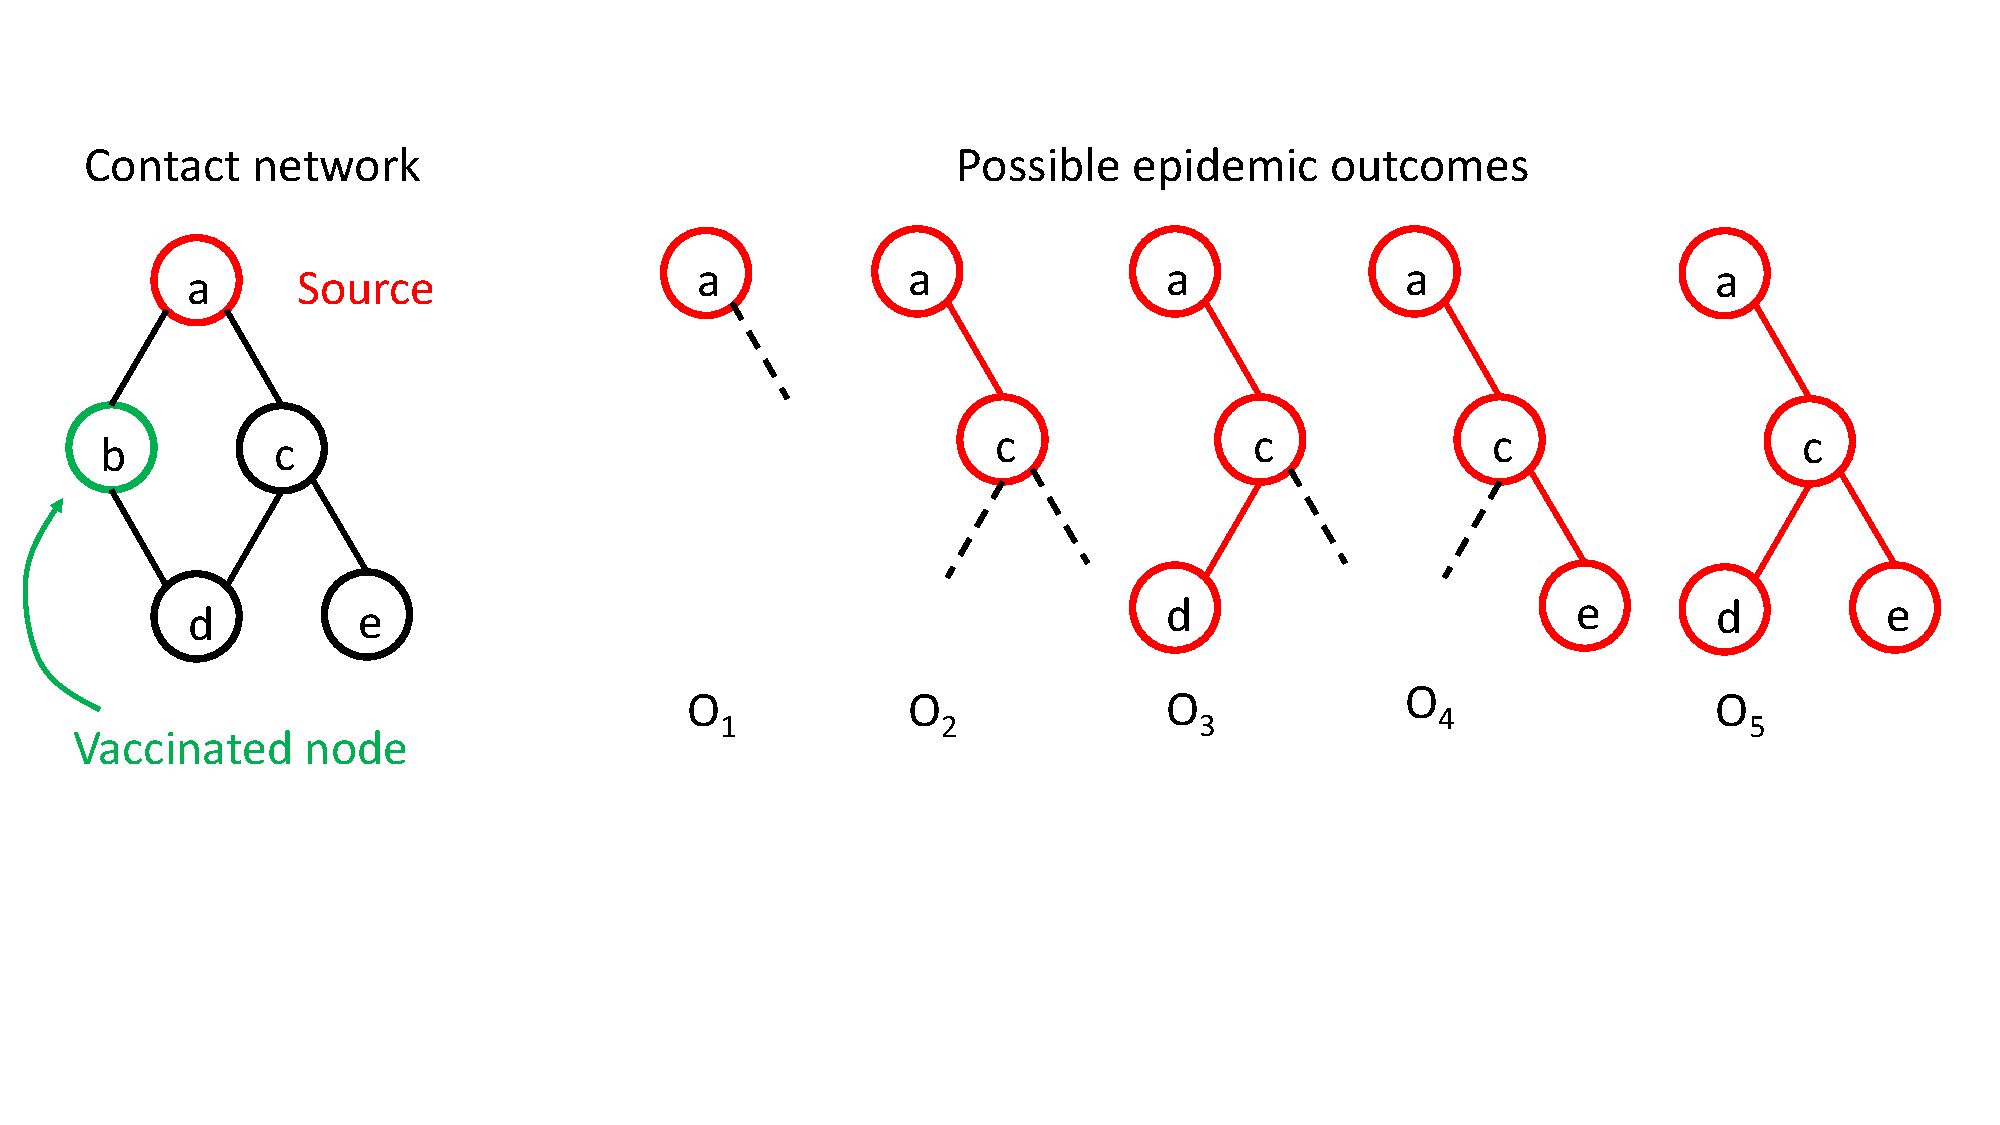
\includegraphics[scale=0.25]{figures/example.pdf}
\caption{Example illustrating the SIR model: the contact network $G=(V, E)$ is shown in the left,
with $V=\{a, b, c, d, e\}$ (shown in circles), and edges as solid lines.
Node $a$ is initially infected, and node $b$ is vaccinated. The five subgraphs $O_1, O_2, O_3, O_4, O_5$
(on the right) are possible stochastic outcomes in the SIR model.}
\label{fig:example}
\end{figure}

\noindent
\textbf{Interventions and objective.}
We use $x_{vt}$ as an indicator variable, which is $1$ if node $v$ gets vaccinated at time $t$.
Let $\X_t=\{v: x_{vt}=1, v\in V\}$ denote the set of nodes vaccinated at time $t$, and 
$\X=\{\X_t: t\in\mathcal{T}\}$ denote the combined set of all temporal vaccination
decisions; here $\mathcal{T}=\{t_0, t_1,\ldots\}$ denotes a set of times at which decisions are to be made.
We assume the vaccine is immediately effective; our methods can be extended to handle limited efficacy vaccines.
We assume a budget vector $\B=(B_t: t\in\mathcal{T})$, which specifies the number of vaccines available
at each time $t\in\mathcal{T}$. We focus on the following objective:
$\expinf(G, \src, \mathcal{T}, \X)$, which denotes the expected number of infections that occur if the epidemic
starts with the vector $\src$, and nodes are vaccinated at each time $t\in\mathcal{T}$, as per the vector $\X_t$.
We use simpler notation to denote the expected number of infections in the following special cases:\\
(1) No vaccination case: $\expinf(G, \src)$, when no vaccinations are done,\\
(2) Single stage: $\expinf(G, \src, \X_0)$, when vaccinations are only done at time 0 for nodes in set $\X_0$, and\\
(3) Two stage: $\expinf(G, \src, \X_0, \X_T)$, when vaccinations are done at two time steps,
namely $0$ and $T$.\\
(4) We drop $G$ and $\src$, when it is clear from the context.

\begin{table}[!h]
\centering
\begin{footnotesize}
\begin{tabular}{|l|l|}
\hline
\textbf{Notation} & \textbf{Definition}\\
$G=(V, E)$ & Graph\\
$\src$ & Source distribution\\
$p$, $p(u, v)$ & Transmission probability\\
$x_{vt}$ & Indicator for node $v$ vaccinated at time $t$\\
$\X_t$ & Set of nodes vaccinated at time $t$\\
$\X$ & Set of all $\X_t$'s\\
$\mathcal{T}$ & Time steps at which intervention is done\\
$\expinf(G, \src, \mathcal{T}, \X)$ & Expected number of infections with intervention $\X$\\
$\expinf(G, \src, \X_0)$ & Exp. \#infections for single stage with intervention $\X_0$\\
$\expinf(G, \src, \X_0, \X_T)$ & Exp. \#infections for two stage version\\
\prob & Designing temporal intervention to minimize $\expinf$\\
\probone & Problem with one stage\\
\probtwo & Problem with two stage\\
$(\alpha, \beta)$ approximation & Bicriteria approximation factor\\
\hline
\end{tabular}
\end{footnotesize}
\caption{Summary of notation used in the paper.}
\label{tab:notation}
\end{table}

\noindent
\textbf{Example.} Figure \ref{fig:example} shows the SIR model and the definitions of the above quantities
on a graph $G$ with five nodes. Initially, node $a$ is infected, and $b$ is vaccinated. 
In the SIR model, the disease spreads from an infected node to each susceptible neighbor with probability $p$,
and does not spread with probability $1-p$. Therefore, we have five possible stochastic outcomes $O_1,\ldots,O_5$,
which occur with probabilities $1-p$, $p(1-p)^2$, $p^2(1-p)$, $p^2(1-p)$, and $p^3$, respectively.
Suppose we have $\mathcal{T}=\{0\}$. Then, $x_{b0}=1$, and $\X=\X_0=\{b\}$.
We have 
\[
\expinf(\X)= (1-p) +2p(1-p)^2+2\cdot 3 p^2(1-p) + 4p^3
\]

\noindent
\textbf{The temporal vaccination problem (\prob).}\\
\underline{Given}: contact network $G=(V, E)$, initial infection vector $\mathbf{s}$, set of times $\mathcal{T}$,
budget vector $(B_t: t\in\mathcal{T})$\\
\underline{Compute}: a set $\X$ of intervention sets at each time, 
such that $\expinf(G, \src, \mathcal{T}, \X)$ is minimized, and $\sum_v x_{vt} \leq B_t$ for all $t\in\mathcal{T}$.

\noindent
\textbf{Special cases of the \prob{} problem.}
\begin{itemize}
\item
\textbf{Single stage vaccination problem (\probone):} given budget $B_0$, choose $\X_0$ such that $|\X_0|\leq B_0$
and $\expinf(G, \src, \X_0)$ is minimized.
\item
\textbf{Two stage vaccination problem (\probtwo):} given budget $B_0, B_T$, choose $\X_0, \X_T$ such that
$|\X_0|\leq B_0$, $|\X_T|\leq B_T$, and $\expinf(G, \src, \X_0, \X_T)$ is minimized.
\end{itemize}

\noindent
\textbf{Bi-criteria approximate solution.}
We say that an intervention $\X=\{\X_t: t\in\mathcal{T}\}$ is an $(\alpha, \beta)$-approximation if:
(1) $|X_t|\leq \alpha B_t$, for each $t$, and
(2) $\expinf(G, \src, \mathcal{T}, \X)\leq \beta \expinf(G, \src, \mathcal{T}, \X^*)$, where
$\X^*$ is an optimal solution to the instance of \prob{}.
We say an algorithm is an $(\alpha, \beta)$-approximation algorithm, if it gives solutions with this factor.

